\documentclass{article}

\usepackage[a4paper, margin=2cm]{geometry}
\usepackage[utf8]{inputenc}
\usepackage[T1]{fontenc}

\usepackage[czech]{babel}
\usepackage{fvextra}
\usepackage{csquotes}
\usepackage{parskip}

\usepackage{float}
\usepackage{amsmath}
\usepackage{siunitx}
\usepackage{graphicx}

\usepackage[hidelinks, unicode, pdfusetitle]{hyperref}

\graphicspath{{images}}

\title{35-4-4 Hroší růže}
\author{Benjamin Swart}

\begin{document}
\maketitle

\section{Komponenty a jádro}

Graf skluzavek můžeme rozdělit na komponenty souvislosti. Každá komponenta má nějaké \textit{jádro}, ve kterém Filip skončí, pokud se z nějakého políčka začne klouzat. Jelikož z každého políčka vede nejvíše jedna skluzavka, tak existuje po výběru startovního políčka jen jedna možná cesta. Jádro může být buď cyklus, nebo políčko, ze kterého nevede žádná skluzavka.

\begin{figure}[ht]
    \centering
    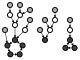
\includegraphics{cores.pdf}
    \caption[Graf skluzavek]{Graf skluzavek. Jádra jsou vyznačeny tmavě šedou, listy jsou vyznačeny světle šedou.}
\end{figure}

Z každého políčka v jádru je možné se dostat na jakékoliv jiné políčko ve stejném jádru.

\section{Souvislé grafy}

Souvislé grafy mají jednu komponentu souvislosti, a díky tomu i jen jedno jádro. Plné dosažitelnosti můžeme dosáhnout jednoduše tak, že postavíme \textit{zpětnou} skluzavku z jádra do každého listu.

\begin{figure}[ht]
    \centering
    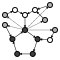
\includegraphics{back-edge.pdf}
    \caption{Nové skluzavky vedoucí z jádra do listů}
\end{figure}

Z každého políčka se pak Filip může snadno dostat do každého jiného tak, že nejprve sjede do jádra, pak vyjede do jednoho z listů podstomu cílového políčka, a nakonec sjede do cíle. Toto řešení postaví tolik skluzavek, jako je v grafu listů. Bude určitě optimální, jelikož řešení určitě nemůže ponechat žádné políčko bez skluzavky, která by v něm končila.

\section{Spojování komponent}

Má-li graf více než jednu komponentu souvislosti, tak je potřeba přidat skluzavky tak, aby se mezi libovolnými dvěma komponentami dalo přepravit. Nejefektivnější způsob, jak to zařídit, je vytvořit cyklus spojující všechny komponenty pomocí \textit{spojovacích} skluzavek. Na to potřebujeme tolik skluzavek, kolik je komponent. (Ledaže je graf souvislý, to pak nepotřebujeme žádnou.) Určitě nepůjde všechny komponenty spojit pomocí méně skluzavek, protože z každé komponenty musí vést minimálně jedna skluzavka.

\begin{figure}[ht]
    \centering
    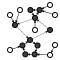
\includegraphics{cross-edge.pdf}
    \caption{Nové skluzavky vedoucí mezi komponentami souvislosti}
\end{figure}

\section{Kombinování principů}

Potřebujeme tedy tolik zpětných skluzavek, jako je listů, a tolik spojovacích skluzavek, jako je komponent. Bohužel ještě nemáme hotovo, protože může být možné, aby jedna skluzavka plnila dvě role.

Spojovací skluzavku, která vede do komponenty s alespoň jedním listem, můžeme postavit \enquote{zdarma} tak, že ji zakončíme v jednom z listů. Do tohoto listu pak nebude muset vést jiná zpětná skluzavka z jádra cílové komponenty.

Touto optimalizací zredukujeme počet skluzavek na počet listů plus počet \textit{holých} jader bez listů. (Jádra složená z jednoho políčka nepovažujeme za listy, i kdyby do nich nevedly žádné skluzavky.) Toto řešení je zjevně optimální, jelikož do každého listu i holého jádra zjevně musí vést skluzavka.

\begin{figure}[ht]
    \centering
    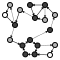
\includegraphics{all-edges.pdf}
    \caption{Vyřešený graf}
\end{figure}

\section{Implementace}

Zbývá jen popsat, jak počítání potřebných skluzavek implementovat. Spočítat listy je snadné, prostě pro každé políčko nejprve spočítáme, kolik v něm končí skluzavek, a potom spočítáme políčka, ve kterých nekončí žádná. Pokud graf obsahuje smyčky, tak je ignorujeme. To zvládneme snadno v čase $\mathcal{O}(n + m) = \mathcal{O}(n)$, protože $m \leq n$. Tím započítáme i holá jádra složená z jednoho políčka, takže nám zbývá jen spočítat holá jádra složená z cyklu dvou nebo více políček.

Počítání cyklů v takovémto grafu není těžké. Stačí vždy začít v nějakém políčku, procházet skluzavky a označovat všechna projetá políčka číslem políčka, ve kterém jsme začali. Pokud narazíme na políčko označené číslem, kterým aktuálně označujeme, tak jsme našli cyklus. Pokud narazíme na políčko označené jiným číslem, tak jsme narazili na prozkoumanou část grafu a můžeme přestat. Postupně se pokusíme začít ve všech políčkách grafu. (Pokud začneme o označeném políčku, tak hned skončíme.) Tento algoritmus také poběží v $\mathcal{O}(n)$.

Celý algoritmus tedy poběží v $\mathcal{O}(n)$ a použije $\mathcal{O}(n)$ paměti.

\end{document}
